\documentclass{icmmcm}

\usepackage[margin=1in]{geometry}
\usepackage{amsmath,amsthm,amssymb}
\usepackage[utf8]{inputenc}
\usepackage{graphicx}
\usepackage{float}
\usepackage{caption}
\usepackage{listings}
\usepackage{subcaption}
\usepackage{appendix}
\usepackage{dirtytalk}
\usepackage{array}
\usepackage[newfloat]{minted}
\usepackage[sorting=none, style=ieee]{biblatex}
\bibliography{references}

\newcolumntype{M}[1]{>{\centering\arraybackslash}m{#1}}
\newenvironment{code}{\captionsetup{type=listing}}{}
% \SetupFloatingEnvironment{listing}{name=Source Code}
\hyphenation{white-space}

\usepackage{color}
\definecolor{codegreen}{rgb}{0,0.6,0}
\definecolor{codegray}{rgb}{0.5,0.5,0.5}
\definecolor{codepurple}{rgb}{0.58,0,0.82}
\definecolor{backcolour}{rgb}{0.95,0.95,0.92}

\newcommand{\fakesection}[1]{%
  \par\refstepcounter{section}% Increase section counter
  \sectionmark{#1}% Add section mark (header)
  \addcontentsline{toc}{section}{\protect\numberline{\thesection}#1}% Add section to ToC
  % Add more content here, if needed.
}
 
\lstdefinestyle{mystyle}{
    backgroundcolor=\color{backcolour},   
    commentstyle=\color{codegreen},
    keywordstyle=\color{magenta},
    numberstyle=\tiny\color{codegray},
    stringstyle=\color{codepurple},
    basicstyle=\footnotesize,
    breakatwhitespace=false,  
    breaklines=true,
    captionpos=b,    
    keepspaces=true,  
    numbers=left,              
    numbersep=5pt,                  
    showspaces=false,                
    showstringspaces=false,
    showtabs=false,
    tabsize=2
}
 
\lstset{style=mystyle}

\title{TU Delft ET4394\\Wireless Networking\\Course Project}
\question{\textbf{LoRa receiver SDR implementation in MATLAB\\using the RTL-SDR dongle}}
\contest{\normalsize{
Guillermo Ortas 4612957
\\Abdul Aziz Hamad 4621565
\\Kumar Navneet 4619110
}}

\begin{document}

\maketitle
\begin{center}

\vspace{32 pt}
March 6, 2017
\end{center}

% \fakesection{Abstract}
%\begin{summary}
%Stuff
%\end{summary}


\textit{Guidelines:\\
I would like to see now in detail (and on paper/code) what have you achieved so far. Please write whatever you have developed/learned/next steps
Upload the report (report source and source code for your implementation) to GitHub (http://github.com) and share the link on Slack. You can also invite me to your repository. Deadline: Thursday, 9 March 9:00 AM (right before the lecture). Report should be compact, so please do not spend a lot of space for writing it - go straight to the point.}


\tableofcontents
% \listoffigures


\newpage
\section{Introduction}
The project aims is to develop a software defined radio RTL-SDR LoRa receiver implemented in MATLAB, using the RTL-SDR USB dongle (RTL2832U) as a radio receiver. LoRa technology refers only to the physical layer of the Low-Power Wide-Area Network (LPWAN) standard, LoRa is completed by LoRaWAN, a media access control (MAC) layer protocol. LoRa uses a proprietary chirp spread-spectrum (CSS) modulation owned by Semtech which enables large distance and low bit rate communications, having in mind IoT devices.

TUDelft is part of The Things Network (TTN), which is an international community aiming to build a global Internet of Things data network which uses the LoRaWAN protocol.
As a member of TTN, TUDelft has a gateway installed on the rooftop of the EEMCS building, which enables communication between devices in the area. This potentially enables us to receive traffic coming from or arriving to this access point. This system is maintained by the professor Fernando Kuipers (Network Architectures and Services).

\section{Initial research}
High level information about this technology is provided by the LoRa Alliance itself and TTN, but information of how it actually works at a lower level is not disclosed due to being a patent pending modulation. Also a lot more information about LoRaWAN can be found than about LoRa.

Luckily, a software engineer from Bastille Research named Matt Knight has lately been working on reverse-engineering the modulation and developing a python open-source for Gnu-Radio implementation of the LoRa physical layer[1]. This implementation is quite well documented and explained on line and it will be used as a reference throughout this whole project. A lot of information and understanding of the inner working of LoRa was extracted from this work.

These are some general and basic but very important points about the modulation to take into account at all times:

\begin{itemize}
    \item The modulation can be understood as a kind of FSK on top of a chirp signal.
    \item The used spreading factor is the number of bits per symbol and ranges from 6 to 12.
    \item The bandwidth of the channels can either be 125 kHz, 250 kHz or 500 kHz.
    \item The chirp rate is $\frac{BW}{2^{SF}}$.
    \item The preamble/training sequence consists of 10 consecutive up-chirps, corresponding to the value zero.
    \item The Start of Frame Delimiter (SFD) is made up of two and a quarter down-chirps, immediately followed by the data.
\end{itemize}


\section{Project organization}
The project is divided in two distinct main blocks: demodulation and decoding. The first block is about translating the raw RF signal into bits and the second block is about processing those acquired bits to actually get the transmitted data out of them.
\subsection{Demodulation block}
This section consists of the following steps:
\begin{enumerate}
    \item Acquire a LoRa signal and isolate signal bandwidth of interest.
    \item De-chirp the signal with a locally generated complex conjugate of the modulating chirp.
    \item Plot the spectrogram of the de-chirped signal with adequate parameters to visualize the transmitted symbols in the resulting frequency modulation.
    \item Since the preamble always carries the value zero, alignment of the data symbols with it is required (modulating and local chirps are most certainly out of phase).
\end{enumerate}
To start working on the demodulation process we could use a prerecorded LoRa sample signal which can be found on line or just capture one of our own using the RTL-SDR dongle.

When plotting the spectrogram, the length of the FFTs should be $2^{SF}$, since there are exactly that many possible symbols. The most powerful component of each FFT corresponds to the transmitted symbol. Overlapping FFTs can be used to reduce confusion and align the data with the SFD.

To align and normalize the symbols to the preamble we should subtract its position from the data symbols and perform a $2^{SF}$ modulo operation to have them in the correct range. After this, we can just directly assing a symbol to each frequency component at a given time instance.

\subsection{Decoding block}
In the encoding process these steps are applied:
\begin{enumerate}
    \item Gray coding.
    \item Whitening.
    \item Interleaving.
    \item Forward Error Correction (FEC).
\end{enumerate}
In order to retrieve the data, these steps must be reversed. Gray coding assigns strings of bits to the symbols, but successive values differ in only one bit. Whitening add randomness and makes the modulation more resilient to noise. An XOR operation is performed to the data against a known sequence. Interleaving shuffles the data before being transmitted to avoid multiple errors in a row, which are more difficult to correct. Finally step 4 uses a Hamming (N,4) code, which encodes 4 bits into N, adding parity bits.

What Matt Knight did was to reduce the number of variables transmit a packet of all zeroes. This means that interleaving does nothing and that FEC just adds more zeroes. Using the reversibility property of the XOR operation he was able to get the whitening sequence, since 0 XOR data = data. The interleaving was harder to crack, but finally he concluded that a diagonal interleaver was used, just with the two most significant bits flipped.

\section{Current progress}
So far we have been researching quite a bit on the topic to become more familiar and understand what is happening under the hood. We have been able to capture various LoRa sample signals at 869.472 MHz using the RTL-SDR dongle in SDR\# from Van Hasseltlaan (student housing complex) which is about 2.3 km away from the TUDelft gateway in a straight line, though the real source of the signal cannot be known for sure (i.e. a device was sending data towards the gateway).

Using MATLAB, we have plotted the spectrogram of the recorded signal with appropriate parameters, it is depicted in Figure \ref{fig:Fig1}.

\begin{figure}[h]
  \begin{center}
    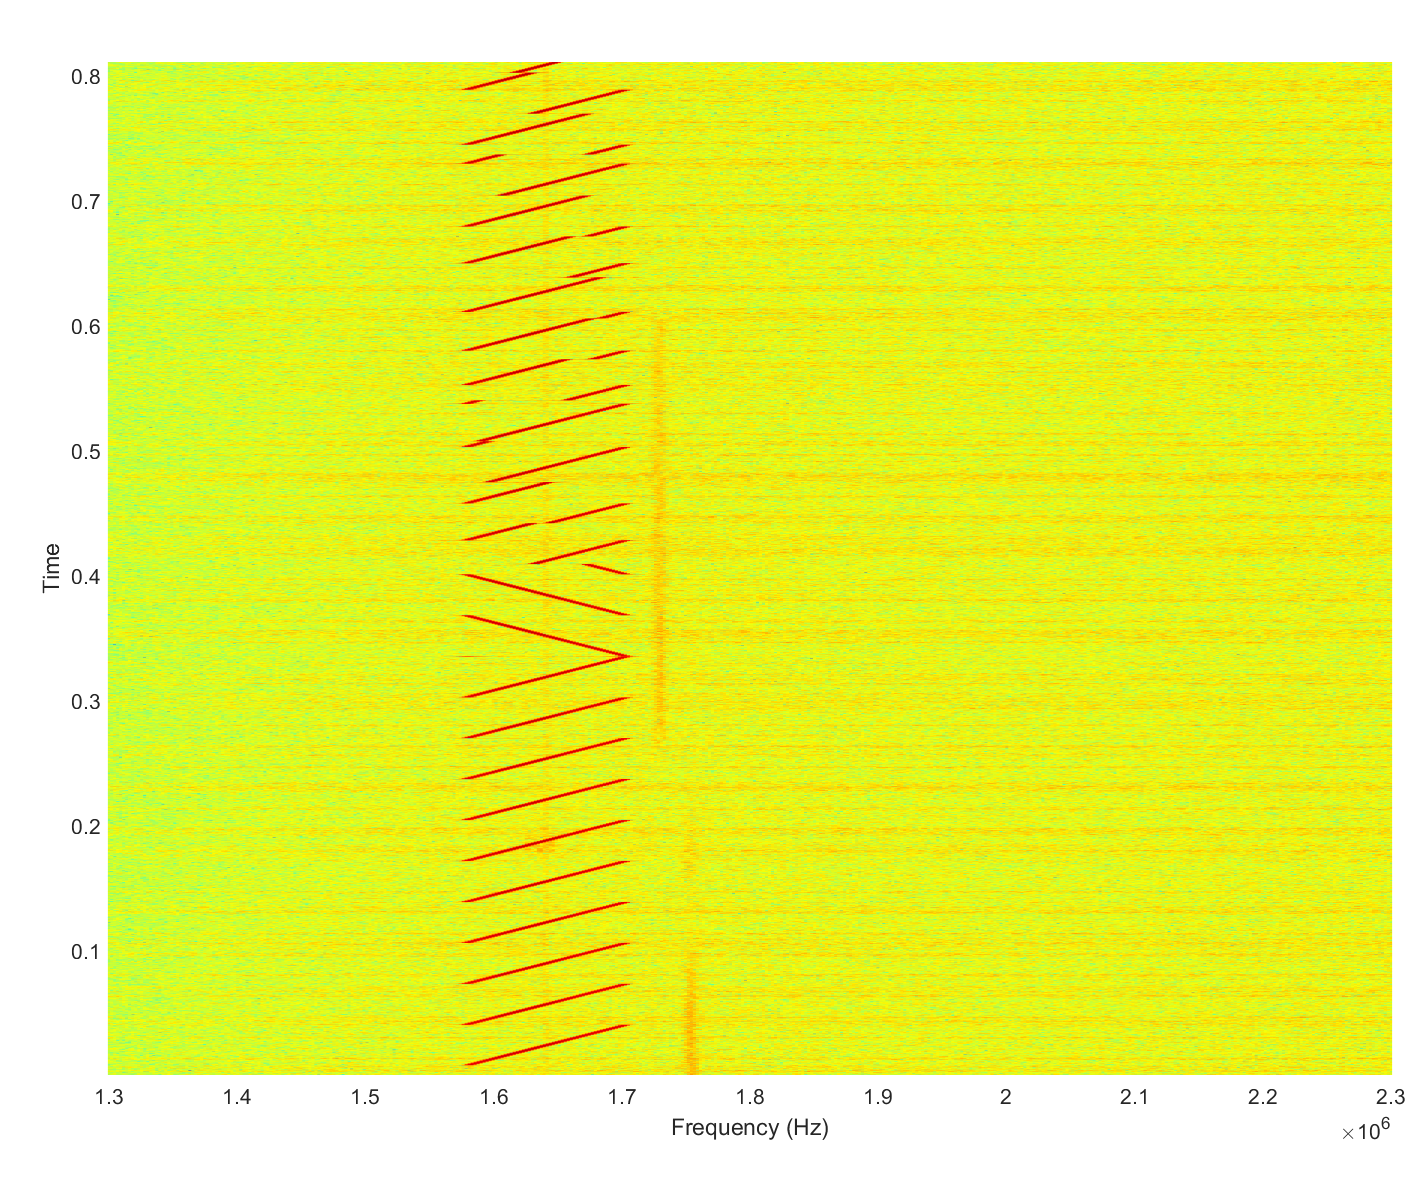
\includegraphics[width=12 cm]{Figures/1}
  \end{center}
  \caption{Spectrogram of the captured LoRa signal.}
  \label{fig:Fig1}
\end{figure}

This specific signal was recorded on March 1 at around 5:30 PM using a rate of 2.4 Ms/s. From the picture we can tell that the used bandwidth is 125 kHz, which was always the case for all observed signals at this frequency. We can also very easily identify the 10 up-chirps of the preamble and the 2.25 down-chirps of the SFD, followed by choppy chirps, which contain the data. The frequency axis refers to the offset from the center frequency of the recording (868.713 MHz) as SDR\# moves it to base-band. We can derive what the spreading factor is from the chirp rate, but we don't know at all what data has been transmitted, which is a downside for the decoding process.

The code for plotting this graph is detailed in Listing \ref{code:spectrogram_plot}.

\begin{code}
\begin{minted}[mathescape, linenos, numbersep=5pt, gobble=2, frame=lines, tabsize=4, framesep=2mm]{matlab}
    close all
    clear all
    
    % Read file
    [in, Fs] = audioread('SDRSharp_20170301_172427Z_868712500Hz_IQ_125k.wav');
    
    % Allocate in-phase and quadrature components
    x = (in(:,1) + 1i*in(:,2))';
    
    % Crop signal in time
    n = 2.306*Fs:4.13*Fs; % values in seconds
    x = x(n);
    
    % Spectrogram parameters
    window_length = 1024;
    Nfft = window_length;
    
    % SPECTROGRAM OPTION 1
    % spectrogram(x, kaiser(window_length), window_length/2, Nfft, Fs);
    
    % SPECTROGRAM OPTION 2
    [s, f, t] = spectrogram(x, kaiser(window_length), window_length/2, Nfft, Fs);
    % f = f(299:352); % crop frequency
    % s = s(299:352,:); % crop spectrogram
    surf(f,t,10*log10(abs(s.')),'EdgeColor','none')
    axis xy; axis tight; colormap(jet); view(0,90);
    ylabel('Time');
    xlabel('Frequency (Hz)');
    % xlim([1.3e6 2.3e6])
    % ylim([0.001 0.81])
\end{minted}
\captionof{listing}{Code for plotting the spectrogram of the recorded signal.}
\label{code:spectrogram_plot}
\end{code}

After this, we were (and still are) working on the generation of the local chirp to multiply the recorded signal with, to get the frequency modulation. The problem we are facing is that we have not been able to generate a band-limited chirp yet. This means that the chirp does not go back and forth in the 125 kHz bandwidth range, but it occupies the whole spectrum instead. This behaviour results in the "de-chirped" signal to show jumps in frequency in steps of 125 kHz, not staying still as it should be. The resulting spectrogram is shown in Figure \ref{fig:Fig2} and it was generated using the code of Listing \ref{code:dechirp_try}.

The less powerful chirp spectral components corresponds to the additional signal that was captured along with the LoRa signal in the recording. This can be solved by filtering beforehand. We can observe that all other chirp parameters that make up the chirp rate and other characteristics are correctly set, as the resulting frequency bins remain straight and constant between jumps when the preamble is transmitted (the transmission of the same symbol would result in a constant frequency when de-chirped).



\begin{figure}[h]
  \begin{center}
    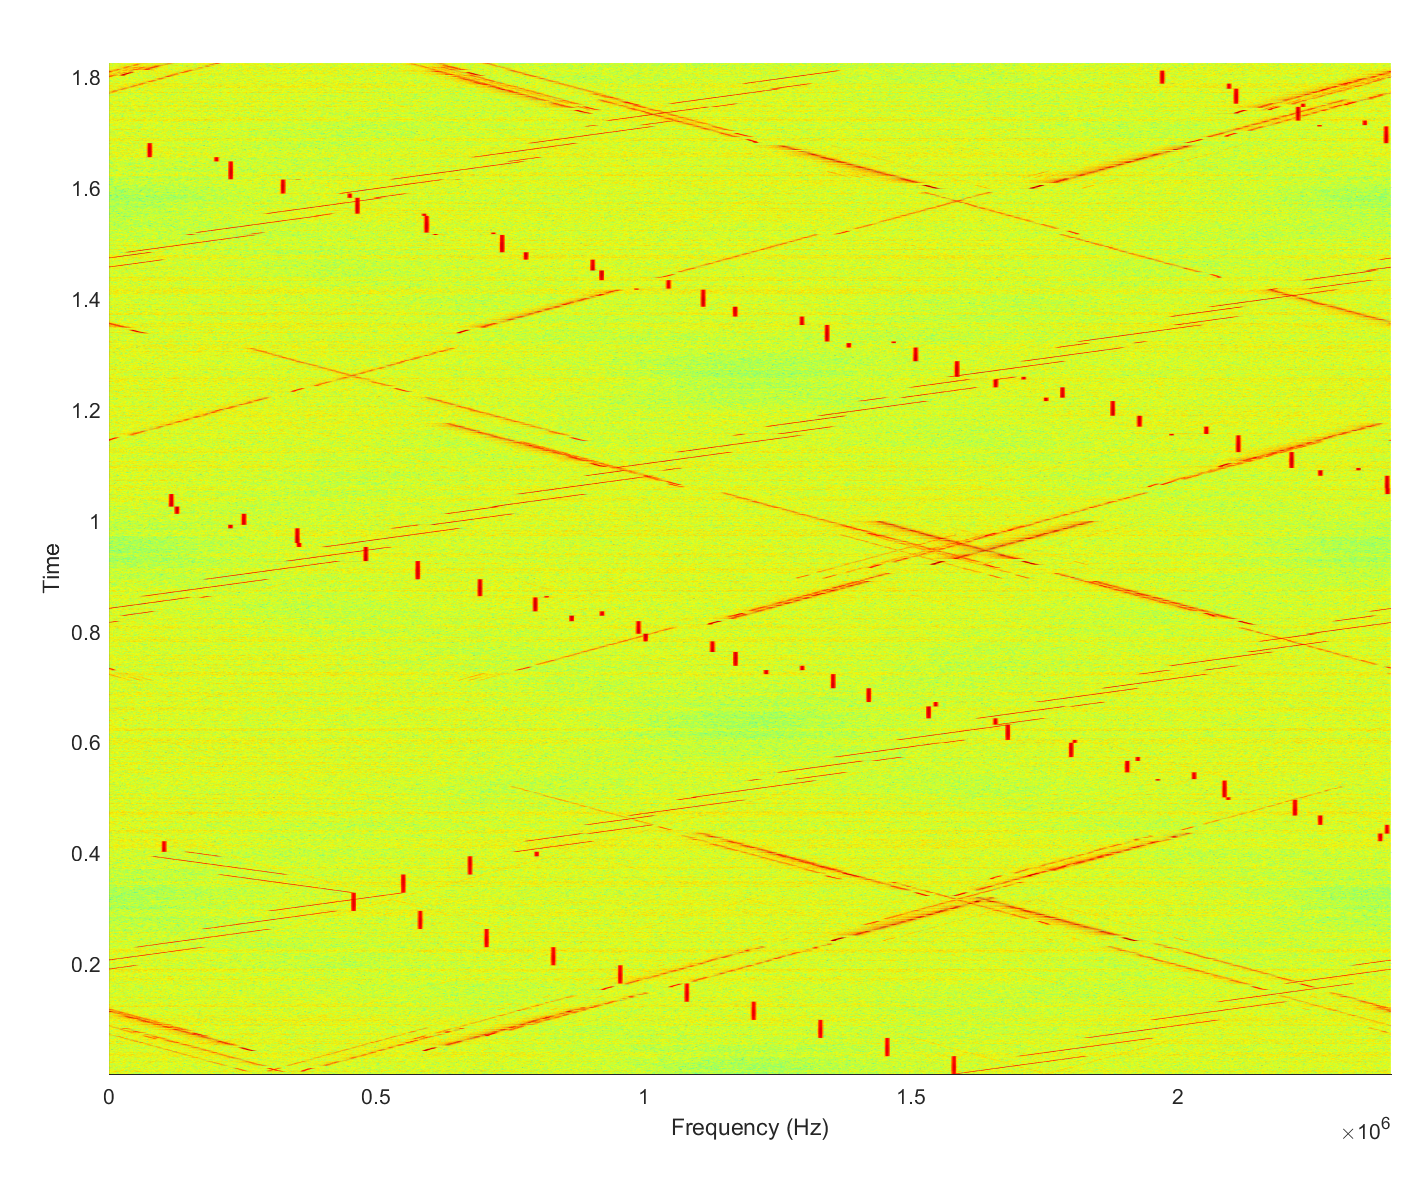
\includegraphics[width=12 cm]{Figures/2}
  \end{center}
  \caption{Spectrogram of first try at de-chirping the recorded signal.}
  \label{fig:Fig2}
\end{figure}

\begin{code}
\begin{minted}[mathescape, linenos, numbersep=5pt, gobble=2, frame=lines, tabsize=4, framesep=2mm]{matlab}
    close all
    clear all
    
    % Read file
    [in, Fs] = audioread('SDRSharp_20170301_172427Z_868712500Hz_IQ_125k.wav');
    
    % Allocate in-phase and quadrature components
    x = (in(:,1) + 1i*in(:,2))';
    
    % Spectrogram parameters
    Nx = length(x);
    window_length = 1024;
    Nfft = window_length;
    % Nfft = 2^SF;
    
    % Crop signal in time
    n = 2.306*Fs:4.13*Fs;
    x = x(n);
    
    % % Test to bring signal to baseband
    % t = 0:1/Fs:length(x)/Fs-1/Fs;
    % x = x.*cos(2*pi*1.577e6*t);
    
    % LoRa parameters
    BW = 125e3;
    SF = 6;
    chip_rate = BW/2^SF;
    Fs_prime = 2*BW;
    
    % Chirp generation
    fo = 0;
    f1 = BW;
    delta_t = 32.8e-3;
    t = 0:1/Fs:length(x)/Fs-1/Fs;
    c = chirp(t,fo,delta_t,f1);
    
    % De-chirping
    de_chirped = x.*conj(c);
    
    % de_chirped = decimate(de_chirped, floor(Fs/2/BW));
    
    % Plot spectrogram
    [s, f, t] = spectrogram(de_chirped, blackman(window_length), window_length/2, Nfft, Fs);
    surf(f,t,10*log10(abs(s')),'EdgeColor','none')
    axis xy; axis tight; colormap(jet); view(0,90);
    ylabel('Time');
    xlabel('Frequency (Hz)');
    % printfigure('Caputred LoRa signal')
    
    % % Plot spectrum
    % X = fft(x, Nfft)/Nfft;
    % f = Fs*linspace(0,1,Nfft);
    % plot(f,10*log10(abs(X)))
    
    % % Test to crop signal in frequency
    % X = X(.5781/(2*pi)*Nfft:.6875/(2*pi)*Nfft);
    % x = ifft(X);
\end{minted}
\captionof{listing}{Code of the first try to de-chirp the recorded signal and plot its spectrogram.}
\label{code:dechirp_try}
\end{code}

\section{Next steps}
We think that the best possible alternative to correctly de-chirp the signal is to just isolate the LoRa signal channel so it occupies the whole bandwidth and then multiply it with the local chirp. We have been thinking about ways to do so, such as cropping the signal in the frequency domain and then take the IFFT, but it seems it's not working properly yet.

For now we are focusing on the de-chirping step. The next steps are to keep working on the de-chirping process and the rest of the demodulation block steps to try and correctly acquire and see the transmitted symbols in the the recorded signal spectrogram. After that, we will move on to the decoding block.

\section{References}
[1] https://github.com/rpp0/gr-lora
[2] 


\end{document}